%\documentclass[preprint,12pt,authoryear]{elsarticle}
\documentclass[final,5p,times,twocolumn]{elsarticle}

\usepackage{amssymb}
\usepackage{amsmath}
\usepackage{subcaption}
\usepackage{algorithmic}
\usepackage{graphicx}
\usepackage{xcolor}
\usepackage{epsfig}
\usepackage{epstopdf}
\usepackage{float}
\usepackage{bm}
\usepackage{kotex}
\usepackage[ruled,vlined]{algorithm2e}
\usepackage{mathtools}
\usepackage{longtable}
\usepackage{booktabs}
\usepackage{url}
\usepackage{tabularx}
\usepackage{array}
\journal{Ocean Engineering}

\begin{document}

\begin{frontmatter}

\title{Cooperative Navigation for Maritime Autonomous Surface Ships through Communication-Enabled Distributed Intelligence}

\author[label1]{Yong Hun Jang}
\author[label1]{Seung Hyun Oh}
\author[label2]{Hoon Lee\corref{cor1}}
\author[label1]{Sang Hyun Lee\corref{cor2}}
\cortext[cor1]{Corresponding author. Department of Electrical Engineering, Ulsan National Institute of Science and Technology, Ulsan, 44919, Korea.}
\cortext[cor2]{Corresponding author. School of Electrical Engineering, Korea University, Seoul 02841, Korea.}

\affiliation[label1]{organization={School of Electrical Engineering, Korea University},
            city={Seoul},
            postcode={02841},
            country={Korea}}

\affiliation[label2]{organization={Department of Electrical Engineering, Ulsan National Institute of Science and Technology},
            city={Ulsan},
            postcode={44919},
            country={Korea}}

\begin{abstract}
{\color{violet}
Cooperative navigation among Maritime Autonomous Surface Ships (MASS) is challenging in partially observable maritime environments, where limited local sensing restricts situational awareness during multi-vessel encounters. This paper develops a communication-enabled cooperative navigation framework for coordinated path planning and collision avoidance. Each vessel encodes its local observation into a compact latent message, while messages from multiple neighboring vessels are combined with their relative geometry and aggregated with the receiving vessel's own observation. A COLREGs-conditioned Mixture-of-Experts (MoE) architecture separates common perception from situation-specific decision making: the radar perception module is shared across encounter experts, while the downstream decision cores are specialized for the corresponding COLREGs situations. Communication is introduced after a local navigation policy has first been established, and an auxiliary threat-decoding objective encourages each transmitted message to retain collision-relevant information observed by its sender.

The framework is evaluated in a GPU-batched maritime simulator with 16 simultaneously navigating vessels. Controlled experiments isolate the effects of inter-vessel communication, shared-perception expert design, multi-neighbor aggregation, message dimensionality, COLREGs shaping, and the timing at which communication is introduced. Communication reduces collision rate and control effort while improving COLREGs compliance, and the shared-perception MoE provides a favorable safety--model-size tradeoff compared with single-network and fully separated alternatives. The results demonstrate that communication-enabled distributed intelligence can improve cooperative navigation under partial observability while retaining decentralized execution.
}
\end{abstract}

\begin{keyword}
Maritime autonomous surface ships \sep Cooperative navigation \sep Inter-vessel communication \sep Collision avoidance \sep COLREGs compliance \sep Multi-agent reinforcement learning
\end{keyword}

\end{frontmatter}

\section{Introduction}
{\color{violet}
The rapid advances of autonomous navigation technologies have brought Maritime Autonomous Surface Ships (MASS) to the forefront of maritime research and regulation. The International Maritime Organization (IMO) has examined the operation of MASS through its regulatory scoping exercise, reflecting growing interest in remotely controlled and fully autonomous vessels \cite{1}. Despite this progress, safe and efficient navigation in congested waters remains a major challenge to the practical deployment of MASS \cite{2}. Autonomous vessels need to avoid collisions while complying with the International Regulations for Preventing Collisions at Sea (COLREGs), particularly in dense maritime traffic where multiple vessels may interact simultaneously under uncertain and changing conditions \cite{3}.

Cooperative navigation involves multiple vessels coordinating their trajectories and sharing locally acquired information to improve navigational safety and efficiency \cite{4}. Each vessel observes only part of the surrounding environment and exchanges locally available information with neighboring vessels. The received information is combined with the vessel's own observation to determine its subsequent navigation behavior. Instead of relying on a complete global representation of the maritime environment, cooperative navigation distributes locally acquired information among vessels so that their trajectories can be coordinated according to surrounding traffic conditions.

Communication-enabled cooperative navigation involves three key operations. First, each vessel extracts navigation-relevant information from its local observation and encodes it into a compact message. Second, messages received from neighboring vessels within communication range are aggregated into a fixed-dimensional cooperative representation. Third, each vessel determines its trajectory by combining this representation with its own local observation. This information exchange extends situational awareness beyond individual sensing ranges and supports coordinated responses to potential conflicts \cite{5,6}. This communication distinguishes cooperative navigation from independent collision avoidance, where surrounding vessels are treated as moving obstacles and each vessel determines its trajectory solely from locally available observations.

Classical path-planning techniques include graph-search algorithms such as A* and Dijkstra's algorithm, sampling-based planners, and artificial potential field methods \cite{8}. Graph-search methods can determine optimal or near-optimal routes with respect to a predefined discretization and cost function, whereas potential-field methods provide computationally efficient local guidance. However, these methods rely on predefined representations of the navigation environment and do not directly resolve the coupled interactions among multiple autonomous vessels \cite{10}. Model Predictive Control (MPC) incorporates vessel dynamics, operational constraints, and short-term motion predictions into online trajectory planning \cite{11}. Its computational cost generally increases with the number of interacting vessels and the prediction horizon, which complicates its application to dense multi-vessel environments \cite{12}. Rule-based methods explicitly encode COLREGs requirements, but their navigation behavior is largely determined by predefined encounter categories and may become difficult to specify for multi-vessel encounter configurations \cite{13}.

Deep reinforcement learning (DRL) provides a learning-based approach to autonomous vessel navigation beyond predefined planning and encounter rules. Through repeated interactions with simulated maritime environments, an autonomous vessel can learn a collision-avoidance policy without explicitly programming every possible encounter and avoidance maneuver \cite{16,17,18}. Existing studies have shown that DRL can jointly account for goal reaching, collision avoidance, and COLREGs compliance within a learned navigation policy \cite{19,20}. However, most single-agent DRL approaches model surrounding vessels as dynamic obstacles rather than cooperative agents. These vessels neither exchange information nor coordinate their trajectories, leaving each agent to navigate solely from observations available within its own sensing range. This formulation limits situational awareness and does not support cooperative collision avoidance.

Cooperative navigation introduces additional learning challenges in multi-agent environments. As the policy of each vessel evolves during training, the transition dynamics observed by one agent change with the policies of other agents, creating a non-stationary learning environment that can destabilize joint policy learning \cite{21}. Partial observability further limits the information available to each vessel \cite{22}. Radar, cameras, and other onboard sensors have finite ranges and fields of view, and their measurements can be affected by occlusion, environmental conditions, and sensor uncertainty \cite{23,24}. As a result, each vessel determines its navigation behavior using incomplete information about the surrounding maritime traffic.

Inter-vessel communication can alleviate partial observability by exchanging information acquired locally by individual vessels \cite{25}. Direct transmission of raw observations, however, increases communication overhead and may convey information irrelevant to the current navigation task. Learned communication instead encodes the local observation of each vessel into a compact, task-relevant message optimized jointly with the navigation policy \cite{26,27}. Communication alone, however, does not ensure effective cooperation. Coordinated navigation depends on the information encoded in each message, the aggregation of messages from a varying number of neighbors, and the use of the aggregated information in selecting navigation actions. These factors become increasingly important in dense maritime traffic, where several vessels may simultaneously enter communication range and create interacting collision risks.

Multi-agent reinforcement learning (MARL) extends reinforcement learning to environments where multiple agents learn and act concurrently \cite{31}. Communication-enabled MARL incorporates the exchange of observations or learned messages to supplement information unavailable from local observations \cite{35}. Existing studies have largely focused on small-scale multi-vessel settings, including two-vessel environments \cite{36}. In a larger encounter, a receiving vessel must combine messages from a varying number of neighbors without making the policy input depend on their order. At the same time, the receiver must preserve enough spatial context to distinguish where each message originates.

COLREGs compliance creates a second form of heterogeneity. A vessel may simultaneously act as a give-way vessel relative to one neighbor and a stand-on vessel relative to another \cite{38,39}. The physical scene is common across these situations, but the appropriate control response is not. This observation motivates the central design principle of this work: \emph{share what is common, specialize what is behaviorally different, and communicate what is locally missing}. Radar perception is therefore shared across COLREGs experts, decision making is specialized by encounter type, and information unavailable from local sensing is exchanged through a compact inter-vessel channel.

Based on this principle, the proposed framework combines three elements. First, each vessel produces a six-dimensional latent message; the receiver attaches relative bearing and distance before aggregating messages from up to four neighbors. Second, a deterministic COLREGs assessment hard-routes the current state to one of five situation-specific decision cores, while the high-dimensional radar encoder is shared among them. Third, PPO updates preserve the gradient path from the receiving vessel's control objective to the MessageActor of the transmitting vessel, and an auxiliary ThreatDecoder encourages the learned message to retain collision-relevant local information. Communication is activated only after an initial local-navigation stage so that the communication channel is learned on top of a stable control policy.

The main contributions of this paper are summarized as follows:
\begin{itemize}
    \item \textbf{Position-grounded multi-neighbor communication:} A compact learned message is combined with sender-relative bearing and distance at the receiver before permutation-invariant aggregation, preserving spatial attribution without requiring the message itself to encode position.

    \item \textbf{Shared-perception, situation-specific decision making:} COLREGs geometry provides a deterministic routing signal. The radar perception module is shared across encounter experts, whereas the downstream decision cores remain situation specific, avoiding unnecessary replication of the parameter-dominant perception network.

    \item \textbf{Communication learning with valid credit assignment:} Partner messages are recomputed during PPO updates from stored partner observations, so the receiver's policy loss can train the sender's MessageActor. A threat-decoding auxiliary objective further regularizes the message representation.

    \item \textbf{Controlled component-wise evaluation:} Communication, expert sharing, neighbor aggregation, message width, COLREGs shaping, and communication-introduction timing are evaluated separately under matched settings, with multi-seed variability reported whenever available.
\end{itemize}

The remainder of this paper is organized as follows. Section 2 introduces the vessel dynamics and COLREGs requirements. Section 3 reviews path-planning and cooperative-navigation methods for MASS. Section 4 presents the proposed framework. Section 5 describes the simulation and evaluation protocols. Section 6 presents the experimental results, and Section 7 concludes the paper.
}

\section{Background}
{\color{violet}
This section describes the vessel motion model and the COLREGs considered for autonomous navigation. The motion model characterizes the kinematic and dynamic behavior of a vessel, while the COLREGs specify the navigation rules for collision avoidance in different encounter situations.
}

\begin{figure}[!t]
    \centering
    \includegraphics[width=.9\linewidth]{figure/fig1}
    \caption{Vessel control model for collision avoidance event.}
    \label{fig:example1}
\end{figure}

\subsection{Vessel Dynamics}
{\color{violet}
Fig.~\ref{fig:example1} shows a vessel control model. A vessel controls its motion through propulsion thrust and rudder angle, represented by the control vector $\boldsymbol{\tau}$. The vessel pose in the earth-fixed frame is defined as $\boldsymbol{\eta}=[x,y,\psi]^T$, where $x$ and $y$ denote the position and $\psi$ denotes the heading angle. The body-fixed velocity vector is defined as $\boldsymbol{v}=[u,v,r]^T$, where $u$, $v$, and $r$ denote surge velocity, sway velocity, and yaw rate, respectively.

The body-fixed velocity is transformed into the earth-fixed frame by the rotation matrix
\begin{equation}
\mathbf{T}(\psi)=
\begin{bmatrix}
\cos\psi & -\sin\psi & 0\\
\sin\psi & \cos\psi & 0\\
0 & 0 & 1
\end{bmatrix},
\end{equation}
and the vessel kinematics are expressed as
\begin{equation}
\dot{\boldsymbol{\eta}}=\mathbf{T}(\psi)\boldsymbol{v}.
\label{eq:kinematics}
\end{equation}
The translational and rotational dynamics can be written in the conventional form
\begin{equation}
\mathbf{M}\dot{\boldsymbol{v}}+\mathbf{C}(\boldsymbol{v})\boldsymbol{v}+\mathbf{D}(\boldsymbol{v})\boldsymbol{v}+\mathbf{g}(\boldsymbol{\eta})=\mathbf{B}\boldsymbol{\tau},
\label{eq:dynamics}
\end{equation}
where $\mathbf{M}$ denotes inertia, $\mathbf{C}(\boldsymbol{v})$ Coriolis and centripetal effects, $\mathbf{D}(\boldsymbol{v})$ hydrodynamic damping, and $\mathbf{B}$ the actuator mapping. The simulator used in this work restricts motion to the horizontal plane and implements the corresponding surge and yaw response using acceleration, deceleration, drag, and rudder-response parameters.
}

\begin{figure}[!t]
    \centering
    \includegraphics[width=\linewidth]{figure/png/fig2}
    \caption{Encounter situations described by COLREGs.}
    \label{fig:example2}
\end{figure}

\subsection{Collision Avoidance and COLREGs}
{\color{violet}
The International Regulations for Preventing Collisions at Sea (COLREGs) specify navigation rules for preventing collisions between vessels. Among these regulations, Rules~13--17 define the principal obligations associated with the encounter situations considered in this study. These situations are illustrated in Fig.~\ref{fig:example2} and summarized below.
\begin{itemize}
    \item \textbf{Overtaking (Rule~13):} An overtaking vessel keeps clear of the vessel being overtaken until it is finally past and clear.
    \item \textbf{Head-On (Rule~14):} When two vessels approach on reciprocal or nearly reciprocal courses, each vessel alters its course to starboard so that they pass on the port side of each other.
    \item \textbf{Crossing (Rule~15):} In a crossing encounter, the vessel that has the other vessel on its starboard side acts as the give-way vessel and keeps clear.
    \item \textbf{Give-Way Vessel (Rule~16):} The give-way vessel takes early and substantial action to keep clear of the other vessel.
    \item \textbf{Stand-On Vessel (Rule~17):} The stand-on vessel maintains its course and speed but may take action to avoid collision when the give-way vessel does not take appropriate action.
\end{itemize}

In a multi-vessel environment, a vessel may simultaneously hold different pairwise obligations relative to several neighbors. Collision risk is commonly characterized by the Distance at Closest Point of Approach (DCPA) and Time to Closest Point of Approach (TCPA). DCPA represents the predicted minimum separation if the current courses and speeds are maintained, whereas TCPA represents the time remaining until that closest approach. These quantities are used by the deterministic encounter assessment introduced later.
}

\section{Related Work}
{\color{violet}
Related studies on MASS navigation can be broadly grouped into path planning and cooperative navigation. Path-planning studies focus on generating feasible routes and collision-avoidance trajectories for individual vessels, while cooperative-navigation studies consider how multiple vessels exchange information and coordinate their trajectories. This section reviews both research directions and identifies the limitations addressed by the proposed framework.
}

\subsection{Path Planning for MASS}
{\color{violet}
MASS path planning determines a sequence of positions and control actions that guide a vessel from its origin to a destination while satisfying navigational constraints. Global path planning identifies waypoints that define the overall route from the origin to the destination, whereas local path planning determines detailed trajectories between consecutive waypoints by accounting for real-time vessel dynamics, surrounding traffic, and collision risks \citep{Yuan}.

Global path-planning methods such as A*, Dijkstra's algorithm, and geodesic-based routing can determine optimal or near-optimal routes when an accurate map of the navigation environment is available \citep{58}. A finer map representation improves route planning but increases the search space and computational cost. Data-driven approaches have used Automatic Identification System (AIS) records to incorporate historical vessel movements and environmental conditions into route planning. Neural-network models have generated fuel-efficient routes in Arctic waters using historical speed, course, and ice-concentration data \citep{119}. LSTM-based models have also predicted intermediate waypoints from vessel turning-point data \citep{120}. These methods improve route generation but do not directly resolve collision risks that emerge during navigation.

Local path planning addresses short-term changes according to nearby traffic and evolving encounter conditions. Artificial potential fields, the dynamic window approach, and model predictive control have been widely studied for real-time collision avoidance \citep{58,Xue2024}. DRL provides a learning-based alternative in which collision-avoidance behavior is acquired from repeated interaction. Existing studies incorporate goal reaching, collision avoidance, and COLREGs compliance into the reward structure, and encounter classifiers have been used to activate situation-specific terms \citep{Zhao-COLREGs}. Despite these advances, most approaches still determine collision-avoidance actions independently for each vessel and do not exchange task-dependent latent information among neighboring vessels.
}

\subsection{Cooperative MASS Navigation}
{\color{violet}
When vessels navigate independently, information about neighboring vessels is obtained primarily through onboard sensing and externally available traffic information such as AIS data. Cooperative navigation supplements this information through inter-vessel communication. Existing studies have considered positional information and collision-risk measures such as CPA \citep{58}, control intentions including rudder commands and speed changes \citep{82}, historical trajectories \citep{29}, and learned latent messages \citep{WangZhao2025}.

\citet{WangZhao2025} applied explicit message passing to cooperative vessel navigation using MADDPG and reported improved collision-avoidance performance over single-agent baselines. However, the study considers a two-vessel environment, where each vessel receives information from only one neighbor. In a multi-vessel environment, a receiving vessel must combine a varying number of messages into a consistent policy input and still preserve which relative direction and distance each message refers to.

The proposed framework addresses this problem through position-grounded multi-neighbor aggregation and a COLREGs-conditioned shared-perception MoE. The encounter type is determined by maritime geometry rather than by a learned router. This deterministic situation index selects the corresponding decision core, while the radar encoder is shared across the experts. The communication path is trained jointly with the receiver by preserving sender-to-receiver gradients during PPO updates.
}

\section{Proposed Framework}
\label{sec:framework}
{\color{red}
The proposed design is based on a simple separation of roles. The physical scene seen by the radar is common regardless of whether the vessel is currently stand-on, give-way, head-on, or overtaking; therefore, perception is shared. The correct navigation response differs across these obligations; therefore, decision making is specialized. Finally, each vessel observes only part of the traffic scene; therefore, information that is locally missing is exchanged between vessels. This \emph{shared--specialized--communicated} decomposition is the organizing principle of the algorithm.
}

\subsection{System Overview}
\label{sec:system_overview}
{\color{red}
Consider $N$ vessels indexed by $i\in\{1,\ldots,N\}$. Every vessel executes the same parameter-shared policy and uses only its own local observation and messages received from nearby vessels. Three neural modules are used: a \textit{MessageActor} that produces an outgoing message, a \textit{ControlActor} that produces rudder and thrust commands, and a Critic used during PPO training. The same COLREGs-conditioned expert structure is used in all three modules.

The communication range is larger than the radar range. In the common experiments, $r_{\mathrm{radar}}=56$~m and $r_{\mathrm{comm}}=420$~m, and at most the four nearest communication partners are retained. Communication can therefore provide information about vessels that are not yet represented by direct radar returns.
}

% The existing framework artwork is retained rather than discarded. Its labels
% should be updated in the final artwork to show: shared RadarEncoder, deterministic
% hard routing, position-grounded mean aggregation, ThreatDecoder, and two-stage
% communication activation.
\begin{figure}[t]
    \centering
    \includegraphics[width=\linewidth]{figure/fig6}
    \caption{Overall cooperative navigation framework. The current artwork is retained from the earlier manuscript and will be relabeled to reflect the shared-perception hard-routed MoE and position-grounded message aggregation described in this section.}
    \label{fig:framework_structure}
\end{figure}

\subsection{Observation and Shared Radar Perception}
\label{sec:observation}
{\color{red}
The simulator maintains, for each vessel, a 369-dimensional raw observation consisting of 360 radar rays, two goal variables, four self-state variables, two position variables used for communication geometry, and one COLREGs situation index. The absolute position is not used as a direct learned policy feature.

Three consecutive 360-ray radar scans are stacked and processed by a circular one-dimensional convolutional encoder. The encoder uses three stride-2 convolutional layers with channel sizes $32$, $64$, and $64$ and kernel sizes $5$, $5$, and $3$, followed by a fully connected projection to a 30-dimensional feature. Rather than writing each convolution separately, we denote the complete radar encoder by
\begin{equation}
\mathbf{z}^{r}_i=E_r(\mathbf{R}_i)\in\mathbb{R}^{30},
\label{eq:radar_simple}
\end{equation}
where $\mathbf{R}_i\in\mathbb{R}^{3\times360}$ is the three-frame radar stack. Circular padding reflects the physical adjacency of the $0^\circ$ and $359^\circ$ rays.

The goal observation contains normalized goal distance and relative bearing, and the self-state contains normalized speed, yaw rate, heading, and rudder angle. The input to the downstream decision core is therefore
\begin{equation}
\mathbf{u}_i=
[\mathbf{z}^{r}_i\|\mathbf{g}_i\|\mathbf{s}_i\|\operatorname{onehot}(c_i)]
\in\mathbb{R}^{41}.
\label{eq:policy_feature}
\end{equation}
The raw environment observation is thus 369-dimensional, while the learned dense core receives the compact 41-dimensional representation after radar encoding.
}

\subsection{COLREGs Situation Assessment and Expert Routing}
\label{sec:colregs_assessment}
{\color{red}
The COLREGs situation is determined from vessel geometry; it is not predicted by a neural gating network. Five routing states are used: None, Head-On, Crossing Stand-On, Crossing Give-Way, and Overtaking. The implementation first removes vessels outside the detection range, vessels already behind the own ship, safely passing pairs, and pairs whose closest approach has already passed. The remaining pair is classified using the standard relative-bearing regions for head-on, crossing, and overtaking encounters. Near the bow axis, reciprocal bearing is used to avoid rapid switching between give-way and stand-on labels.

For every valid pair $(i,j)$, a normalized collision-risk score combines current distance, TCPA, and DCPA. Using $r_d$, $r_t$, and $r_c$ for the three normalized risk components, the implemented score can be summarized as
\begin{equation}
\rho_{ij}=\operatorname{clip}_{[0,1]}
\left[\beta_{c_{ij}}
\left(0.3r_d+0.4r_t+0.3r_c\right)\right].
\label{eq:risk_simple}
\end{equation}
The situation coefficients are 2.0 for Head-On, 1.5 for Give-Way, 1.3 for Stand-On, and 1.2 for Overtaking. The normalized distance, TCPA, and DCPA scales use 56~m, 30~s, and 24~m, respectively. The dominant encounter is simply
\begin{equation}
j_i^*=\arg\max_j \rho_{ij},\qquad c_i=c_{i j_i^*}.
\label{eq:dominant_pair}
\end{equation}
If no valid risky pair exists, $c_i$ is None.

This deterministic routing is used as a domain-informed inductive bias. COLREGs encounter class is already defined by maritime geometry, so the network does not need to rediscover it from data. The neural network learns the control behavior within each situation rather than learning both the situation definition and the control response simultaneously.
}

\subsection{Shared-Perception Mixture of Experts}
\label{sec:shared_moe}
{\color{red}
A fully separated MoE would duplicate the complete radar network for every situation. This is inefficient because radar perception accounts for most of the parameters. Across the MessageActor, ControlActor, and Critic, RadarEncoder parameters account for 328,794 of the 369,131 parameters in the single-network configuration, or approximately 89\%.

The proposed MoE therefore shares perception and specializes only the downstream decision core. For each neural module $q$, the computation is written in the familiar encoder--expert form
\begin{equation}
\mathbf{h}^{(q)}_i
=F^{(q)}_{c_i}
\left(
[E^{(q)}_r(\mathbf{R}_i)\|\mathbf{x}^{(q)}_i]
\right),
\label{eq:moe_simple}
\end{equation}
where $E^{(q)}_r$ is one radar encoder shared across the five experts of that module and $F^{(q)}_{c_i}$ is the decision core selected by the current COLREGs situation. The MessageActor, ControlActor, and Critic each have their own shared radar encoder; the encoder is shared across situations, not across these three modules.

For the MessageActor, the selected core outputs a six-dimensional bounded message,
\begin{equation}
\mathbf{m}_i=M_{c_i}(\mathbf{u}_i)\in[-1,1]^6.
\label{eq:message_simple}
\end{equation}
The ControlActor uses a 128-unit situation-specific hidden layer followed by a 64-unit layer and a two-dimensional action head. The two continuous outputs are normalized rudder and thrust commands and are sampled using a standard squashed-Gaussian PPO policy.

\begin{table}[t]
\centering
\caption{Network structures used in the MoE comparison. Parameter counts include MessageActor, ControlActor, and Critic.}
\label{tab:moe_arch}
\small
\setlength{\tabcolsep}{3pt}
\begin{tabularx}{\columnwidth}{>{\raggedright\arraybackslash}X c r}
\toprule
\textbf{Structure} & \textbf{Decision cores} & \textbf{Params.}\\
\midrule
Single network & 1 & 369,131\\
Separate, thin & 5 & 363,004\\
Separate, full & 5 & 1,826,719\\
\textbf{Shared perception} & \textbf{5} & \textbf{511,543}\\
\bottomrule
\end{tabularx}
\end{table}

The thin separated model narrows internal channels to approximately match the parameter count of the single network. The full separated model keeps the original width and therefore shows the cost of duplicating perception. The proposed model keeps full-width perception but shares it across the five situation-specific decision cores.
}

\subsection{Position-Grounded Multi-Neighbor Communication}
\label{sec:message_passing}

% The earlier message-passing artwork is also retained. It remains useful as a
% layout basis, but the final labels should replace sum aggregation by the
% position-grounded encoding and masked mean below.
\begin{figure}[t]
    \centering
    \includegraphics[width=\linewidth]{figure/fig7}
    \caption{Message-passing architecture retained from the earlier manuscript as the basis for the final revised artwork. The implemented receiver first attaches relative geometry to each learned message and then uses masked-mean aggregation.}
    \label{fig:arch}
\end{figure}

{\color{red}
A latent message tells the receiver \emph{what} the sender has encoded, but a multi-vessel controller also needs to know \emph{where} that information comes from. The receiver can compute relative position directly, so the six-dimensional communication channel does not need to spend capacity on position encoding.

For sender $j$ and receiver $i$, the relative geometry is represented by
\begin{equation}
\mathbf{r}_{ij}=
\left[\sin\phi_{ij},\cos\phi_{ij},d_{ij}/r_{\mathrm{comm}}\right].
\label{eq:relpos_simple}
\end{equation}
The receiver combines this three-dimensional geometry with the six-dimensional sender message,
\begin{equation}
\mathbf{e}_{ij}=f_{\mathrm{msg}}
\left([\mathbf{m}_j\|\mathbf{r}_{ij}]\right),
\label{eq:grounded_message}
\end{equation}
where $f_{\mathrm{msg}}$ is a small $9\rightarrow32\rightarrow6$ network. Up to the four nearest valid messages are then aggregated by a masked mean,
\begin{equation}
\bar{\mathbf{m}}_i=
\frac{1}{|\mathcal{P}_i|}
\sum_{j\in\mathcal{P}_i}\mathbf{e}_{ij},
\label{eq:mean_message}
\end{equation}
with $\bar{\mathbf{m}}_i=\mathbf{0}$ when no communication partner is available. This form is permutation invariant while preserving spatial attribution before aggregation.

The ControlActor and Critic each multiply the aggregated message by a learnable scalar gate before using it. The gate is initialized at a neutral value rather than fully closed. This provides the network with the representational ability to down-weight unhelpful communication without assuming that finite training must always make communication beneficial.
}

\subsection{Learning the Communication Channel}
\label{sec:comm_learning}
{\color{red}
The communication path is useful only if the receiving vessel's objective can train the message generator of the sending vessel. During data collection, the rollout buffer therefore stores the observations of the selected communication partners rather than only storing their already-generated messages. During each PPO update, the partner messages are recomputed by the current MessageActor and aggregated again using Eqs.~\eqref{eq:relpos_simple}--\eqref{eq:mean_message}. The receiver's policy loss can consequently propagate through the aggregated message to the sender's MessageActor.

A second auxiliary objective encourages the six-dimensional message to retain information that is useful to another vessel. The three nearest threats observed by the sender are represented by bearing, distance, and closing-rate information. A small decoder maps the six-dimensional message to these threat descriptors. Instead of introducing a long element-wise expression, the auxiliary objective is written as the standard masked reconstruction loss
\begin{equation}
\mathcal{L}_{\mathrm{th}}
=\operatorname{MaskedMAE}
\left(D_{\mathrm{th}}(\mathbf{m}_i),\mathbf{y}^{\mathrm{th}}_i\right),
\label{eq:threat_simple}
\end{equation}
where $D_{\mathrm{th}}$ is a $6\rightarrow64\rightarrow12$ decoder for up to three four-dimensional threat descriptors. The coefficient used in the common experiments is $0.5$. This loss shapes what information remains available in the message but does not directly prescribe the receiver's action.

The message-producing and message-consuming layers are initialized with small nonzero weights. This avoids the zero-gradient product that occurs when both sides of the communication path start exactly at zero. The rollout also stores the pre-$\tanh$ sampled action so that the PPO likelihood used during the update is consistent with the action that was actually sampled.
}

\subsection{Reward and PPO Training}
\label{sec:training}
{\color{red}
The reported Fig.~1--Fig.~8 checkpoints use the same Standard reward generation. Rather than expressing every dense term as a separate equation, the reward is grouped into four familiar components,
\begin{equation}
R_i=R_i^{\mathrm{task}}+R_i^{\mathrm{safety}}+R_i^{\mathrm{eff}}+R_i^{\mathrm{COLREGs}}.
\label{eq:reward_grouped}
\end{equation}
The first term rewards arrival and goal progress, the second penalizes collision and risky proximity, the third discourages unnecessary time and control effort, and the last introduces directional COLREGs behavior. Table~\ref{tab:reward} lists the implemented coefficients used to generate the principal experimental checkpoints.

\begin{table*}[t]
\centering
\caption{Standard reward terms used by the reported experimental checkpoints.}
\label{tab:reward}
\small
\begin{tabularx}{\textwidth}{p{0.20\textwidth} p{0.28\textwidth} X}
\toprule
\textbf{Term} & \textbf{Coefficient / form} & \textbf{Role}\\
\midrule
Arrival & $+100$ terminal & Reward successful arrival\\
Collision & $-300$ terminal & Strong safety penalty\\
Time & $-0.07$ & Discourage unnecessarily long navigation\\
Forward motion & $+0.1(v_i/v_{\max,i})$ & Maintain forward motion\\
Low-speed penalty & $-0.15$ when active & Avoid stationary behavior\\
Control effort & $-0.02[(v_i/v_{\max,i})^2+0.5a_{\delta,i}^2]$ & Penalize large thrust/turning effort\\
Near proximity & linear penalty inside 19.6~m & Penalize close approach\\
Collision course & $-0.8\rho_i$ & Penalize the dominant collision risk\\
Pairwise risk & $-0.3\sum_j\rho_{ij}^{1.6}$ & Penalize simultaneous risks\\
Far-field shaping & $0.5(F_i(t-1)-F_i(t))$ & Encourage reduction of 56--420~m far-field risk\\
Goal progress & $d_{g,i}(t-1)-d_{g,i}(t)$ & Reward movement toward the goal\\
Goal heading & $0.15\cos\theta_{g,i}(v_i/v_{\max,i})$ & Favor goal-aligned motion\\
Rudder smoothness & $-0.02|\Delta\delta_i|/30^\circ$ & Suppress abrupt steering\\
COLREGs & coefficient $0.45$ & Penalize directionally noncompliant maneuvers when risk is high\\
\bottomrule
\end{tabularx}
\end{table*}

The COLREGs term is intentionally simple in interpretation. When the dominant risk exceeds 0.3, Head-On, Give-Way, and Overtaking encounters penalize a port-side avoidance command, whereas Stand-On penalizes unnecessary steering. Its magnitude is scaled by $(1+\rho_i)$ and coefficient $0.45$. This acts as a domain prior that breaks the symmetric failure mode in which two cautious vessels independently choose incompatible avoidance directions.

The policy is optimized with PPO and generalized advantage estimation. The implemented loss can be written in the conventional form
\begin{equation}
\mathcal{L}
=\mathcal{L}_{\mathrm{PPO}}
+0.5\mathcal{L}_V
-0.01\mathcal{H}
+0.5\mathcal{L}_{\mathrm{th}},
\label{eq:ppo_simple}
\end{equation}
where $\mathcal{L}_{\mathrm{PPO}}$ is the standard clipped PPO policy loss, $\mathcal{L}_V$ is the value loss, and $\mathcal{H}$ is policy entropy. The clip parameter is 0.2, $\gamma=0.99$, GAE $\lambda=0.95$, learning rate is $3\times10^{-4}$, two PPO epochs are used per rollout, minibatch size is 512, and gradient norm is clipped at 0.5.

The main training runs use a two-stage communication schedule within the same 16-million-decision run. Incoming communication is zero until 9 million decisions; from that point onward the learned communication path is activated without reinitializing the policy. The COLREGs coefficient remains 0.45 throughout. This schedule separates learning a basic local control law from learning how to exploit a communication channel whose representation is itself changing during training.
}

\section{Simulation Environment and Evaluation Protocol}
\label{sec:simulation}

\subsection{GPU-Batched Maritime Simulator}
{\color{red}
The numerical experiments are trained and evaluated in the GPU-batched simulator \texttt{vessel\_gym.py}. The simulator reproduces the vessel motion, radar sensing, collision geometry, COLREGs situation logic, and observation contract of the Unity/C\# reference implementation while avoiding the synchronous Unity--Python training bottleneck. Unity remains useful for visualization and reference behavior, but the figures reported in the numerical section are generated from the batched simulator.

The arena is $600\times600$~m with nine circular obstacles of radius 20~m arranged on a $3\times3$ grid with 120~m spacing. The reference scene contains 20 spawn points on an outer square and 16 goal points on an inner square. A ring factor of 0.7 is used in the common experiments. Each environment contains 16 vessels. The initial heading is directed toward the assigned goal with a random perturbation within $\pm10^\circ$, and the maximum speed of each vessel is independently scaled by a factor sampled from $\mathcal{U}(0.8,1.8)$.

Physics is integrated at 0.04~s with ten substeps per policy decision, so the action is updated every 0.4~s. The base maximum speed after simulation scaling is 1.0~m/s. Rudder command is bounded by $30^\circ$ with a physical slew rate of $12^\circ$/s. Vessel collision uses a body footprint of approximately 14.183~m by 1.927~m. Goal arrival is declared within 3~m.

\begin{table}[t]
\centering
\caption{Common configuration for the principal Fig.~1--Fig.~6 experiments.}
\label{tab:env_params}
\small
\setlength{\tabcolsep}{3pt}
\begin{tabularx}{\columnwidth}{>{\raggedright\arraybackslash}X >{\centering\arraybackslash}p{0.31\columnwidth}}
\toprule
\textbf{Parameter} & \textbf{Value}\\
\midrule
Vessels per environment & 16\\
Parallel training environments & 128\\
Arena & $600\times600$~m\\
Obstacle layout & $3\times3$, radius 20~m\\
Ring factor & 0.7\\
Radar range & 56~m\\
Communication range & 420~m\\
Maximum message partners & 4\\
Message dimension & 6\\
Radar frames & 3\\
Environment observation & 369D\\
Physics step / policy decision & 0.04~s / 0.4~s\\
Episode limit & 16,000 physics steps\\
Goal threshold & 3~m\\
COLREGs coefficient & 0.45\\
Threat-decoder coefficient & 0.5\\
Communication activation & 9M of 16M decisions\\
Training seeds & 42, 43, 44\\
\bottomrule
\end{tabularx}
\end{table}
}

\subsection{Evaluation Protocol}
{\color{red}
Each primary comparison changes one axis while leaving the remaining settings fixed. After training, each checkpoint is frozen and evaluated with 96 parallel environments, a 1,500-decision burn-in period, and 3,500 subsequent evaluation decisions. The reported fixed-policy metrics include arrival, collision and timeout rates, fuel/control-effort accumulation, total heading travel, minimum separation, episode length, and overall and situation-specific COLREGs compliance.

Learning curves and fixed-policy bars use different estimators. The curve shown in the experiment folders uses the outcome score
\begin{equation}
J_{\mathrm{curve}}
=1.5P_{\mathrm{arrival}}-6P_{\mathrm{collision}}-0.5P_{\mathrm{timeout}},
\label{eq:curve_simple}
\end{equation}
weighted by the number of completed episodes in each logging window. It should therefore be interpreted as a learning diagnostic rather than as the same quantity reported by the fixed-policy bar plots.
}

\section{Results and Discussion}
\label{sec:results}
{\color{red}
The result sequence follows the algorithm design itself. We first ask whether communication helps at all, then how situation specialization should be structured, how several neighbor messages should be combined, how much message capacity is needed, how COLREGs prior knowledge changes behavior, and when the communication channel should be introduced during training. The final two experiments examine heterogeneous communication capability and route-level A* integration.
}

\subsection{Communication: Is the Shared Information Useful?}
\label{sec:comm_result}
{\color{red}
The first experiment compares the same shared-perception architecture with communication disabled and enabled. Collision rate decreases from 2.77\% to 1.83\%, while overall COLREGs compliance increases from 48.4\% to 52.3\%. Fuel/control-effort accumulation decreases from 816 to 802 and total heading travel from $1930^\circ$ to $1852^\circ$. Arrival rate changes only modestly, from 54.4\% to 55.6\%.

The situation-wise result clarifies where communication is useful. Head-On compliance is already nearly saturated without communication, whereas Give-Way improves from 53\% to 65\% and Stand-On from 21\% to 30\%. Overtaking decreases from 76\% to 70\%; this reversal is retained rather than hidden by the average. The result therefore supports a more specific interpretation than ``communication improves everything'': its strongest benefit appears in encounters in which coordinated intent is less evident from local sensing alone.
}

\begin{figure*}[t]
\centering
\begin{subfigure}{0.32\textwidth}
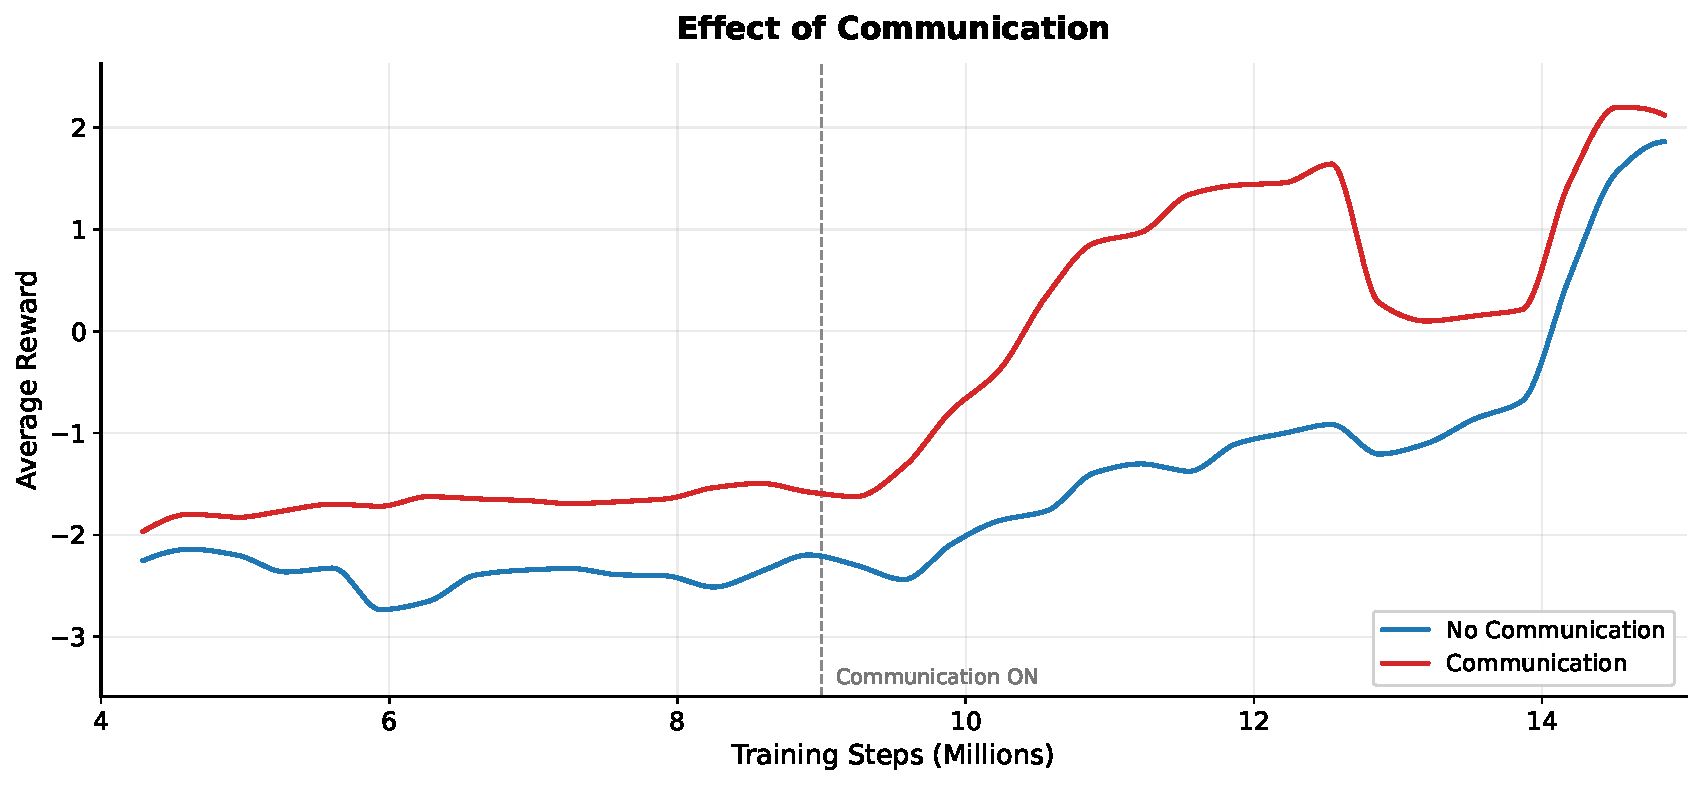
\includegraphics[width=\linewidth]{Fig1_Communication/0_reward_curve}
\caption{Learning outcome score.}
\end{subfigure}\hfill
\begin{subfigure}{0.32\textwidth}
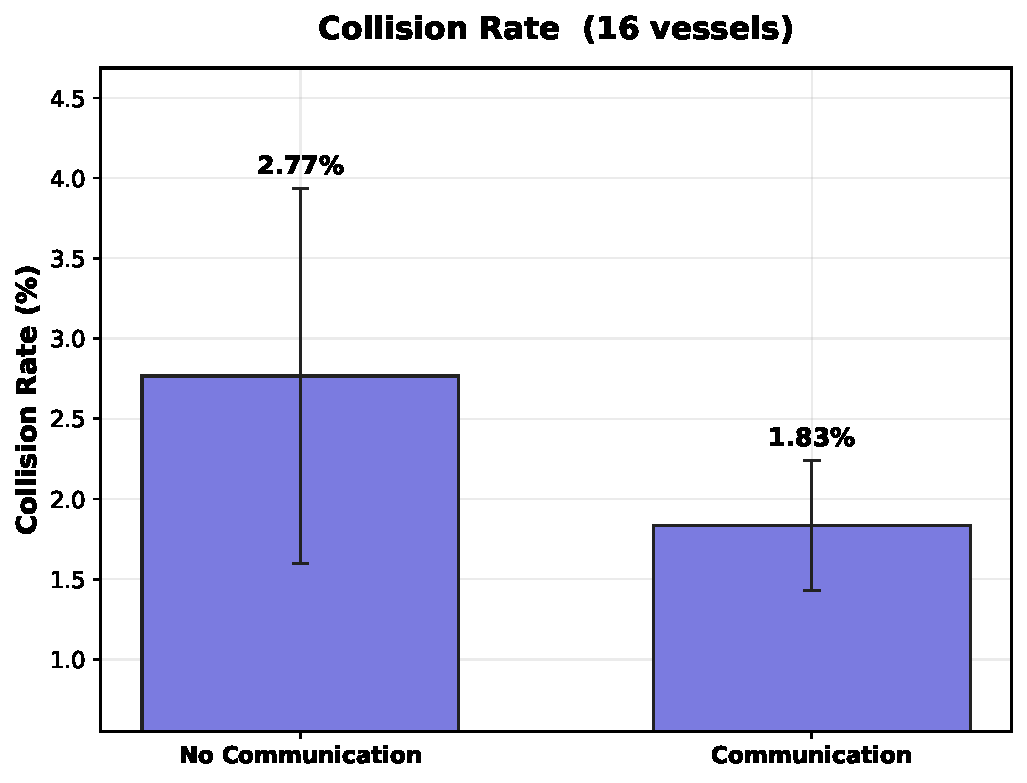
\includegraphics[width=\linewidth]{Fig1_Communication/3_collision_rate}
\caption{Collision rate.}
\end{subfigure}\hfill
\begin{subfigure}{0.32\textwidth}
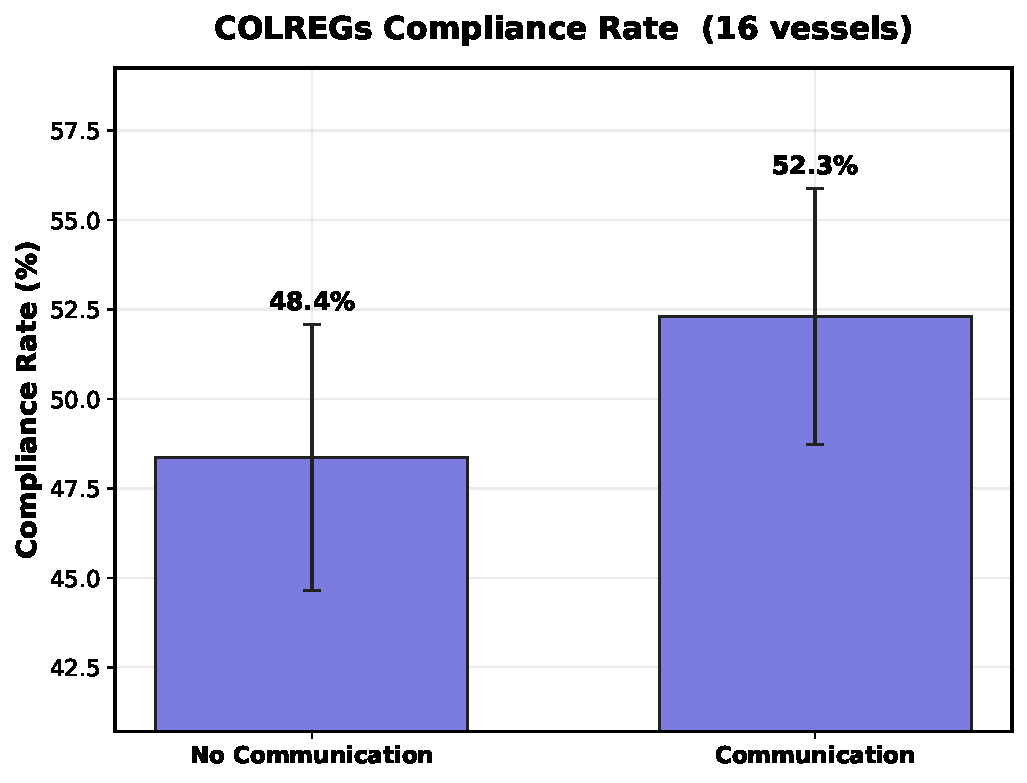
\includegraphics[width=\linewidth]{Fig1_Communication/1_colregs_compliance}
\caption{Overall COLREGs compliance.}
\end{subfigure}\\[4pt]
\begin{subfigure}{0.32\textwidth}
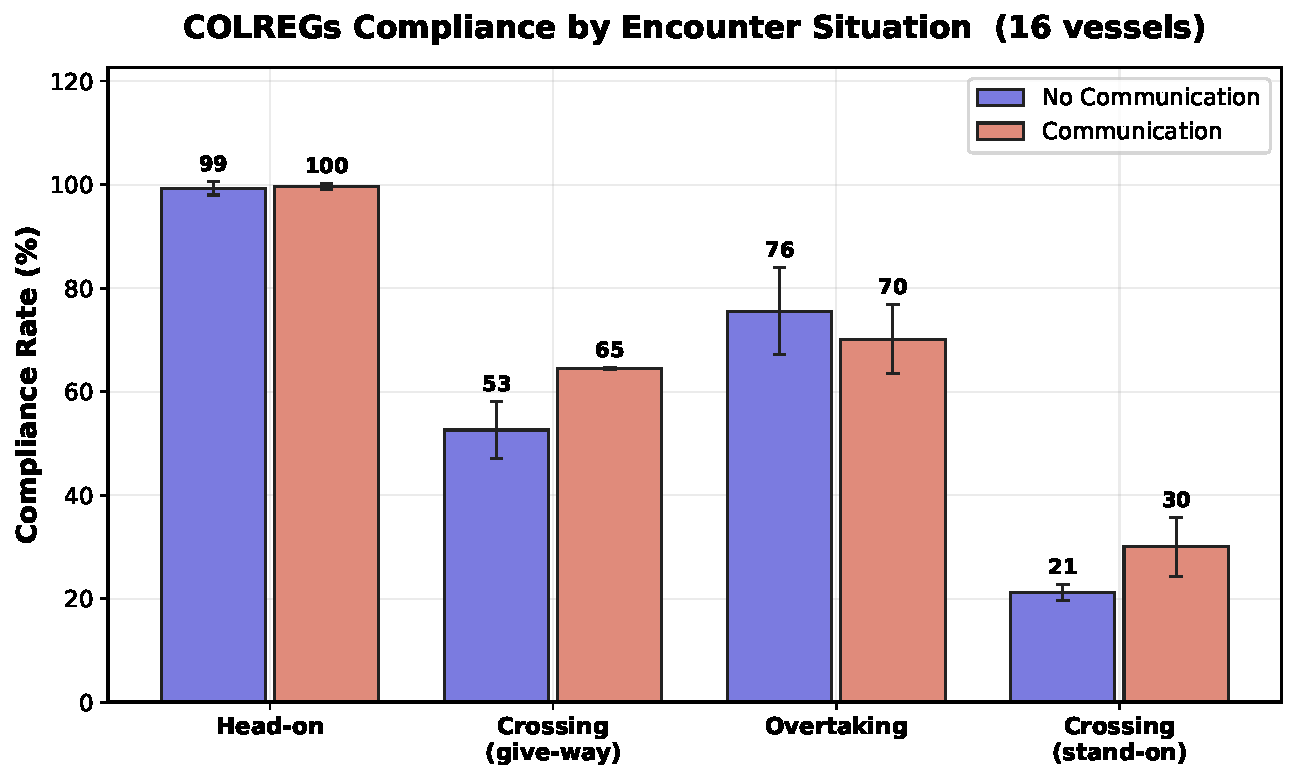
\includegraphics[width=\linewidth]{Fig1_Communication/2_colregs_by_situation}
\caption{Compliance by situation.}
\end{subfigure}\hfill
\begin{subfigure}{0.32\textwidth}
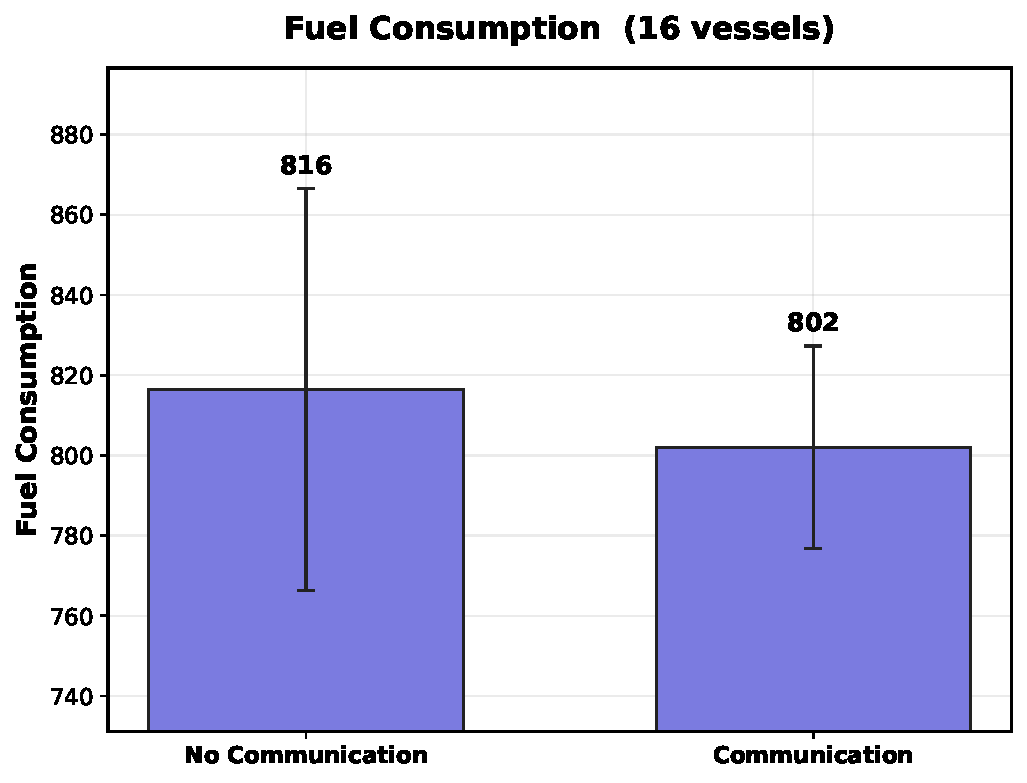
\includegraphics[width=\linewidth]{Fig1_Communication/4_fuel_consumption}
\caption{Fuel/control-effort accumulation.}
\end{subfigure}\hfill
\begin{subfigure}{0.32\textwidth}
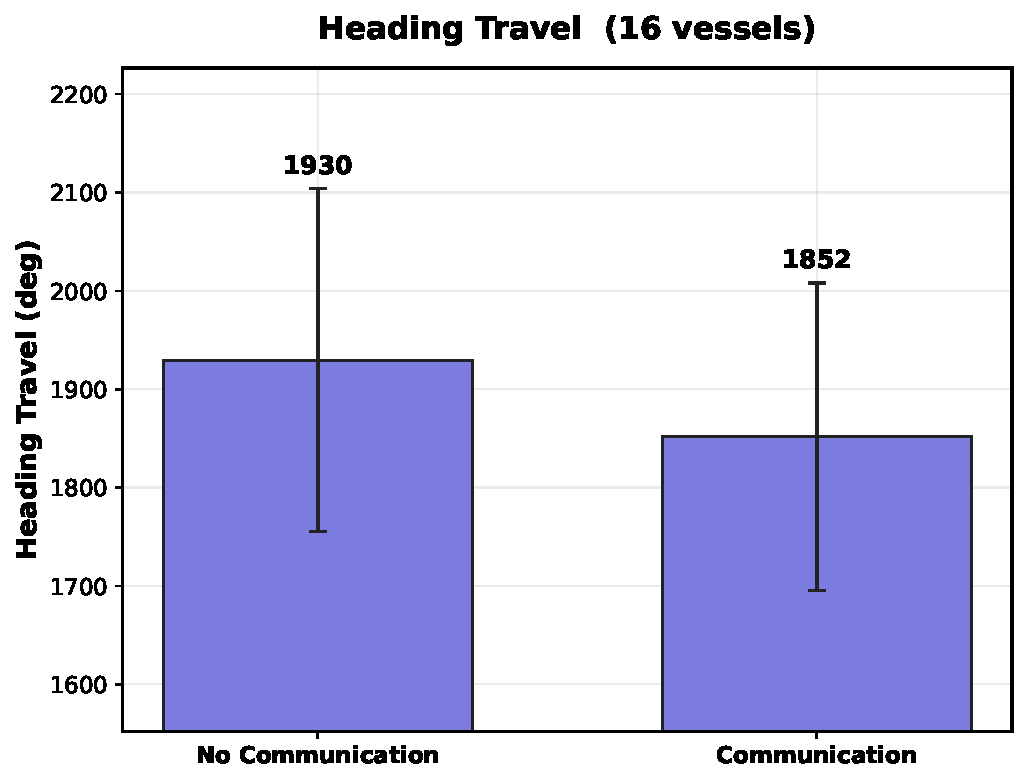
\includegraphics[width=\linewidth]{Fig1_Communication/5_heading_travel}
\caption{Heading travel.}
\end{subfigure}
\caption{Effect of inter-vessel communication. Existing experimental plots are retained and combined into one figure rather than discarded. Communication mainly improves safety, COLREGs coordination, and maneuvering efficiency, while the encounter-wise panel shows that the benefit is not uniform across all COLREGs situations.}
\label{fig:exp_comm}
\end{figure*}

\subsection{MoE Architecture: What Should Be Shared and What Should Be Specialized?}
\label{sec:moe_result}
{\color{red}
This comparison evaluates a single network, a parameter-matched thin separated MoE, a full-width separated MoE, and the proposed shared-perception MoE. The single model contains 369,131 parameters, the thin separated model 363,004, the full separated model 1,826,719, and the proposed model 511,543.

The single model reaches 57.2\% arrival with a 6.07\% collision rate. The thin separated model collapses to 33.8\% arrival and 9.50\% collision. The proposed shared-perception model reaches 55.6\% arrival with only 1.83\% collision. Existing full-separated runs provide the fourth comparison arm; they are kept because they show that simply duplicating full perception is not a free substitute for sharing it. The full-separated model also has somewhat lower fuel and heading travel than the proposed model, so the conclusion is not that shared perception is numerically best on every metric. The stronger claim is that it offers the most favorable combination of safety and model size.

The thin separated condition currently has one completed seed, whereas the other main conditions have three; this limitation is disclosed rather than hidden.
}

\begin{figure*}[t]
\centering
\begin{subfigure}{0.24\textwidth}

\includegraphics[width=\linewidth]{Fig2_MoE_Architecture/0_reward_curve}
\caption{Learning score.}
\end{subfigure}\hfill
\begin{subfigure}{0.24\textwidth}

\includegraphics[width=\linewidth]{Fig2_MoE_Architecture/3_collision_rate}
\caption{Collision rate.}
\end{subfigure}\hfill
\begin{subfigure}{0.24\textwidth}

\includegraphics[width=\linewidth]{Fig2_MoE_Architecture/1_colregs_compliance}
\caption{COLREGs compliance.}
\end{subfigure}\hfill
\begin{subfigure}{0.24\textwidth}

\includegraphics[width=\linewidth]{Fig2_MoE_Architecture/4_fuel_consumption}
\caption{Fuel/control effort.}
\end{subfigure}
\caption{Comparison of MoE structures. The existing plots are retained; the final version will add the full-width separated arm consistently to all panels and pair these results with the parameter counts in Table~\ref{tab:moe_arch}.}
\label{fig:exp_moe}
\end{figure*}

\subsection{Multi-Neighbor Aggregation: Why More Than the Nearest Vessel?}
\label{sec:aggregation_result}
{\color{red}
The aggregation experiment changes only the maximum number of retained communication partners from the nearest one vessel to the nearest four vessels. Four-neighbor aggregation reduces collision rate from 3.43\% to 1.83\%, increases overall COLREGs compliance from 45.6\% to 52.3\%, and reduces both fuel/control effort and heading travel. Situation-specific compliance improves in all four active encounter classes.

The result matches the structural motivation for multi-neighbor communication. A nearest-one controller can resolve the currently closest encounter while simultaneously moving toward another vessel whose message has been omitted. Aggregating several spatially grounded messages lets the policy respond to the local traffic configuration instead of solving a sequence of disconnected pairwise problems.
}

\begin{figure*}[t]
\centering
\begin{subfigure}{0.24\textwidth}

\includegraphics[width=\linewidth]{Fig3_Message_Aggregation/0_reward_curve}
\caption{Learning score.}
\end{subfigure}\hfill
\begin{subfigure}{0.24\textwidth}

\includegraphics[width=\linewidth]{Fig3_Message_Aggregation/3_collision_rate}
\caption{Collision rate.}
\end{subfigure}\hfill
\begin{subfigure}{0.24\textwidth}

\includegraphics[width=\linewidth]{Fig3_Message_Aggregation/1_colregs_compliance}
\caption{Overall compliance.}
\end{subfigure}\hfill
\begin{subfigure}{0.24\textwidth}

\includegraphics[width=\linewidth]{Fig3_Message_Aggregation/2_colregs_by_situation}
\caption{Compliance by situation.}
\end{subfigure}
\caption{Nearest-one versus four-neighbor position-grounded aggregation. The existing experimental plots are retained as a compact four-panel figure.}
\label{fig:exp_aggregation}
\end{figure*}

\subsection{Message Dimension: How Much Capacity Is Needed?}
\label{sec:dimension_result}
{\color{red}
The message-width sweep uses $|\mathbf{m}|\in\{2,4,6,8,10,12\}$. This sweep was performed with the full-width separated MoE rather than the proposed shared-perception architecture, so it is interpreted as a channel-capacity sensitivity study rather than a direct ablation of the final architecture.

Very small messages, particularly dimensions 2 and 4, degrade performance. The outcome score is highest at dimension 8, but the results from dimensions 8 to 12 are not monotonic. The appropriate conclusion is therefore that a moderate latent width is sufficient and that further enlargement does not produce a systematic gain. Dimension 6 is retained in the common experiments to keep the main comparisons matched and the communication vector compact.
}

\begin{figure*}[t]
\centering
\begin{subfigure}{0.24\textwidth}

\includegraphics[width=\linewidth]{Fig4_Message_Dimension/0_reward_curve}
\caption{Learning score.}
\end{subfigure}\hfill
\begin{subfigure}{0.24\textwidth}

\includegraphics[width=\linewidth]{Fig4_Message_Dimension/3_collision_rate}
\caption{Collision rate.}
\end{subfigure}\hfill
\begin{subfigure}{0.24\textwidth}

\includegraphics[width=\linewidth]{Fig4_Message_Dimension/1_colregs_compliance}
\caption{COLREGs compliance.}
\end{subfigure}\hfill
\begin{subfigure}{0.24\textwidth}

\includegraphics[width=\linewidth]{Fig4_Message_Dimension/2_colregs_by_situation}
\caption{Compliance by situation.}
\end{subfigure}
\caption{Sensitivity to message dimension. The sweep supports a moderate-capacity communication channel but does not justify claiming a unique optimal dimension.}
\label{fig:exp_dimension}
\end{figure*}

\subsection{COLREGs Shaping: Domain Knowledge as a Coordination Prior}
\label{sec:colregs_result}
{\color{red}
The matched shared-perception comparison changes only the COLREGs coefficient from 0 to 0.45. In the matched three-seed result, compliance increases from approximately 31.4\% to 52.3\% and collision rate decreases from approximately 6.43\% to 1.83\%. The mechanism is as important as the numerical gain: the COLREGs term gives otherwise symmetric collision-avoidance policies a common directional convention. Head-On, Give-Way, and Overtaking discourage a port-side avoidance response, while Stand-On discourages unnecessary course changes.

The original Fig.~5 plot is retained below as a temporary visualization because it contains usable qualitative structure, but its no-COLREGs arm was generated with a different architecture/seed balance. It must be regenerated from the matched shared-perception three-seed runs before submission. Keeping the plot in the working manuscript avoids discarding useful artwork while preventing its current numbers from being treated as the final controlled comparison.
}

\begin{figure*}[t]
\centering
\begin{subfigure}{0.32\textwidth}

\includegraphics[width=\linewidth]{Fig5_COLREGs_Term/1_colregs_compliance}
\caption{Overall compliance.}
\end{subfigure}\hfill
\begin{subfigure}{0.32\textwidth}

\includegraphics[width=\linewidth]{Fig5_COLREGs_Term/3_collision_rate}
\caption{Collision rate.}
\end{subfigure}\hfill
\begin{subfigure}{0.32\textwidth}

\includegraphics[width=\linewidth]{Fig5_COLREGs_Term/5_heading_travel}
\caption{Heading travel.}
\end{subfigure}
\caption{Temporary visualization of the COLREGs-term experiment. The final version will preserve this layout but regenerate the panels from the matched proposed-architecture three-seed comparison.}
\label{fig:exp_colregs}
\end{figure*}

\subsection{Communication Timing: Why Introduce the Channel Later?}
\label{sec:timing_result}
{\color{red}
Both timing conditions use communication by the end of training and both are trained for 16 million decisions. One condition enables communication from the first update; the other keeps incoming messages zero until 9 million decisions. Delayed activation produces a higher learning score (2.12 versus 1.06), lower collision rate (1.83\% versus 6.53\%), and higher COLREGs compliance (52.3\% versus 46.4\%). Communication from the start produces higher mean arrival (61.3\% versus 55.6\%), but with much larger seed-to-seed spread, approximately $\pm14.5$ percentage points versus $\pm1.4$.

The result therefore supports a safety-and-stability interpretation rather than a claim that every metric improves. Establishing a local control policy first reduces the number of moving representations that must be learned simultaneously when the inter-vessel channel becomes active.
}

\begin{figure*}[t]
\centering
\begin{subfigure}{0.24\textwidth}

\includegraphics[width=\linewidth]{Fig6_Comm_Timing/0_reward_curve}
\caption{Learning score.}
\end{subfigure}\hfill
\begin{subfigure}{0.24\textwidth}

\includegraphics[width=\linewidth]{Fig6_Comm_Timing/3_collision_rate}
\caption{Collision rate.}
\end{subfigure}\hfill
\begin{subfigure}{0.24\textwidth}

\includegraphics[width=\linewidth]{Fig6_Comm_Timing/1_colregs_compliance}
\caption{COLREGs compliance.}
\end{subfigure}\hfill
\begin{subfigure}{0.24\textwidth}

\includegraphics[width=\linewidth]{Fig6_Comm_Timing/2_colregs_by_situation}
\caption{Compliance by situation.}
\end{subfigure}
\caption{Effect of communication-introduction timing. The learning curve and fixed-policy safety metrics show the advantage of learning local control before coupling the agents through the learned channel.}
\label{fig:exp_timing}
\end{figure*}

\subsection{Heterogeneous Communication Capability}
\label{sec:mixed_result}
{\color{red}
The mixed-fleet experiment freezes the trained policy and disables transmission for an increasing number of the 16 vessels while leaving reception available. This directly tests whether the learned controller degrades gracefully when communication capability is heterogeneous.

The existing plots are intentionally retained because the experiment itself remains valuable. However, the archived raw-data bundle currently does not reproduce the exact delivered curves and appears to contain a different seed count. For this reason, Fig.~\ref{fig:exp_mixed} is treated as a provisional visualization and is not used for the main numerical claims until the provenance mismatch is resolved.
}

\begin{figure*}[t]
\centering
\begin{subfigure}{0.32\textwidth}

\includegraphics[width=\linewidth]{Fig7_통통배/1_colregs_compliance}
\caption{COLREGs compliance.}
\end{subfigure}\hfill
\begin{subfigure}{0.32\textwidth}

\includegraphics[width=\linewidth]{Fig7_통통배/3_collision_rate}
\caption{Collision rate.}
\end{subfigure}\hfill
\begin{subfigure}{0.32\textwidth}
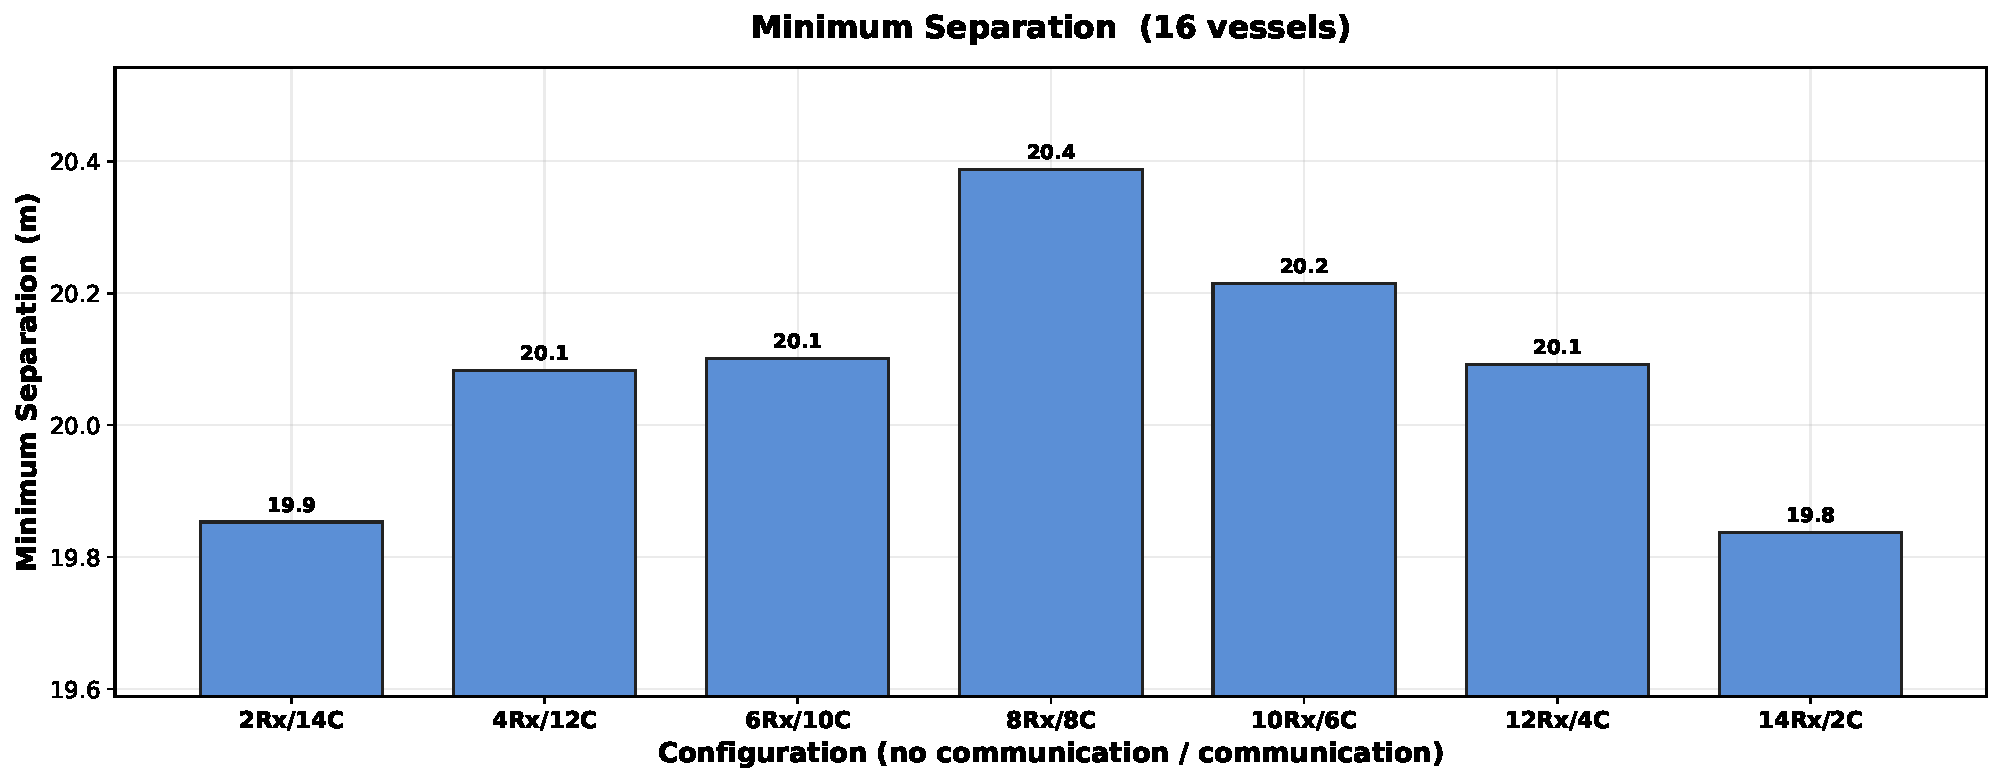
\includegraphics[width=\linewidth]{Fig7_통통배/2_min_separation}
\caption{Minimum separation.}
\end{subfigure}
\caption{Provisional heterogeneous-fleet evaluation with receive-only vessels. The figure is retained in the working manuscript, but its final numerical interpretation is deferred until the delivered plots and archived raw data are reconciled.}
\label{fig:exp_mixed}
\end{figure*}

\subsection{Integration with Global A* Guidance}
\label{sec:astar_result}
{\color{red}
The learned local policy can be coupled to a route-level A* planner by replacing the direct destination with a sequence of collision-free waypoints. The A* route generator has been checked over all 20 spawn points and 16 goals: no generated path intersects the inflated obstacle region, and the final waypoint equals the intended goal in all 320 combinations. The path-to-straight-line ratio has median 1.000 and maximum 1.074.

A separate map demonstrates the same route-generation procedure on a real coastline. The map is a geographic route-planning demonstration, not an AIS-driven traffic digital twin. A final performance comparison still requires rerunning the direct-versus-A* evaluation with the proposed checkpoint and the common ring factor 0.7. This comparison should report both all 320 origin--goal pairs and the 148 pairs for which the straight path is actually blocked, because 172 pairs already have a clear direct line. The current local policy was trained with direct goals, so the A* experiment is a zero-shot waypoint integration unless explicit waypoint-conditioned retraining is performed.
}

\begin{figure}[t]
\centering
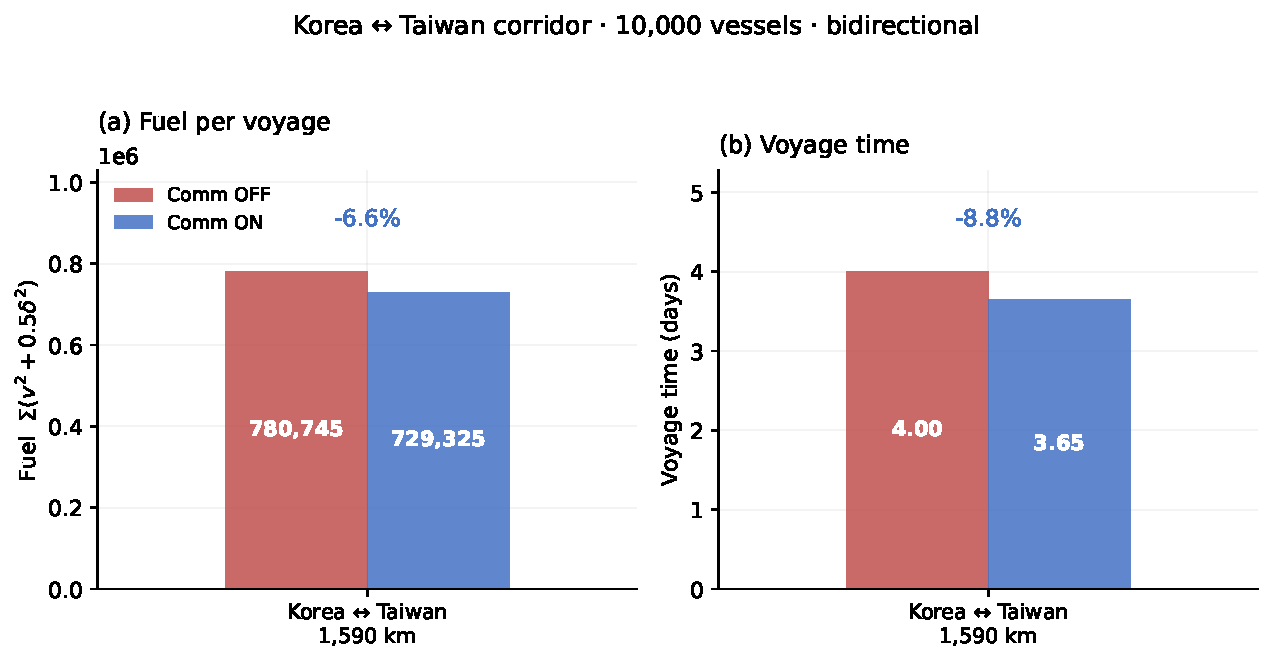
\includegraphics[width=\linewidth]{Fig8_A_/Fig8_korea_taiwan}
\caption{Example global route generated from a real-coastline occupancy map. The map demonstrates route-level path generation; the learned cooperative collision-avoidance policy is trained in the controlled simulator.}
\label{fig:astar_map}
\end{figure}

\subsection{Existing Analyses Retained for Regeneration}
{\color{red}
The previous manuscript also contained fleet-size scalability, a representative trajectory comparison, and t-SNE analysis. These analyses remain useful, but their existing numerical values were produced from an earlier experimental generation. They are therefore not presented as current results. The corresponding artwork and code are retained in the repository and should be regenerated from the same proposed checkpoints used above rather than deleted. The intended replacements are: fixed-policy evaluation at 4, 8, and 16 vessels; a matched communication-ON/OFF trajectory under the 56~m radar and 420~m communication configuration; and t-SNE computed from the current six-dimensional messages and the current observation contract.
}

% ---------------------------------------------------------------------
% Retained old figure blocks for regeneration. They are deliberately kept
% in the manuscript source instead of being deleted.
%
% \begin{figure}[t]
%   \centering
%   \includegraphics[width=\linewidth]{figure/fig5_vessel_number_scalability}
%   \caption{Previous fleet-size scalability artwork; regenerate with the unified checkpoint before reactivating.}
% \end{figure}
%
% \begin{figure}[t]
%   \centering
%   \includegraphics[width=\linewidth]{figure/fig2_scenario_1_overlay}
%   \caption{Previous trajectory-comparison artwork; regenerate under 56~m radar and 420~m communication ranges before reactivating.}
% \end{figure}
%
% \begin{figure}[t]
%   \centering
%   \includegraphics[width=\linewidth]{figure/fig3_tsne_combined}
%   \caption{Previous t-SNE artwork; regenerate from the current six-dimensional message representation before reactivating.}
% \end{figure}
% ---------------------------------------------------------------------

\section{Conclusion}
{\color{red}
This paper presented a communication-enabled cooperative navigation framework for multi-vessel autonomous navigation under partial observability. Its central design principle is to separate what should be shared, what should be specialized, and what must be communicated. Radar perception is shared because all COLREGs situations describe the same physical sensing problem. Decision cores are specialized because stand-on, give-way, head-on, and overtaking impose behaviorally different obligations. Information unavailable from a vessel's local sensing is communicated through a compact learned message whose physical origin is supplied explicitly by the receiver.

This decomposition also explains the empirical results. Shared perception avoids replicating the parameter-dominant radar encoder across five experts while preserving situation-specific control. Position-grounded aggregation allows several neighbor messages to influence one control decision without making the policy input depend on neighbor ordering. Explicit sender-to-receiver credit assignment makes the communication path trainable by the receiver's navigation objective, and delayed communication activation reduces the optimization instability of learning local control and inter-vessel semantics simultaneously.

In the common 16-vessel evaluation, communication reduces collision rate from 2.77\% to 1.83\% while improving COLREGs compliance and reducing fuel/control effort and heading travel. Four-neighbor aggregation reduces collision from 3.43\% to 1.83\% relative to nearest-one communication. The matched COLREGs comparison shows that the directional rule prior reduces collision from approximately 6.43\% to 1.83\% while increasing compliance from approximately 31.4\% to 52.3\%. Delaying communication until after local navigation has been learned further improves safety and substantially reduces inter-seed variability.

Future work will incorporate communication latency, loss, and bandwidth constraints, train explicitly with route-level waypoint sequences, and evaluate the resulting system using higher-fidelity maritime traffic and vessel models. The remaining mixed-fleet and A* performance figures will be finalized only after their raw-data provenance and checkpoint matching are fully aligned with the common experimental protocol.
}

\section*{Acknowledgement}
%This work was supported in part by the National Research Foundation of Korea (NRF) funded by the Ministry of Science and ICT (MSIT), Korea Government under Grant 2022R1A5A1027646, and in part by the Institute of Information and Communications Technology Planning and Evaluation (IITP) through MSIT (Intelligent 6G Wireless Access System) under Grant 2021-0-00467.

\section*{Nomenclature}
\begin{table*}[t]
\centering
\caption{Main notation used in the proposed framework.}
\label{tab:notation}
\small
\begin{tabularx}{\textwidth}{p{0.16\textwidth} X p{0.16\textwidth} X}
\toprule
\textbf{Symbol} & \textbf{Description} & \textbf{Symbol} & \textbf{Description}\\
\midrule
$N$ & Number of vessels & $\mathbf{R}_i$ & Three-frame radar stack\\
$\mathbf{z}^{r}_i$ & Learned radar feature & $c_i$ & Dominant COLREGs situation\\
$\mathbf{m}_i$ & Six-dimensional transmitted message & $\bar{\mathbf{m}}_i$ & Aggregated received message\\
$\mathcal{P}_i$ & Up to four communication partners & $\mathbf{r}_{ij}$ & Relative geometry of sender $j$ to receiver $i$\\
$\rho_{ij}$ & Pairwise collision-risk score & $j_i^*$ & Dominant-risk neighbor\\
$\mathbf{a}_i$ & Rudder/thrust action & $\mathcal{L}_{\mathrm{th}}$ & Threat-decoder auxiliary loss\\
$\gamma$ & Discount factor & $\lambda$ & GAE parameter\\
\bottomrule
\end{tabularx}
\end{table*}

\begin{thebibliography}{00}

\bibitem[Zhang et al., 2022]{Zhang}
Zhang, X., Fu, X., Xiao, Z., Xu, H. and Qin, Z., 2022. Vessel trajectory prediction in maritime transportation: current approaches and beyond. \textit{IEEE Trans. Intel. Trans. Sys.}, 23(11), pp.19980-19998.

\bibitem[Akdağ et al., 2022]{Akdag}
Akdağ, M., Solnør, P. and Johansen, T.A., 2022. Collaborative collision avoidance for maritime autonomous surface ships: a review. \textit{Ocean Engin.}, 250, p.110920.

\bibitem[Deng et al., 2021]{Deng}
Deng, Y., Sheng, D. and Liu, B., 2021. Managing ship lock congestion in an inland waterway: a bottleneck model with a service time window. \textit{Trans. Policy}, 112(1), pp.142-161.

\bibitem[U.S. Commandant, 1999]{COLREGs-USA}
U.S. Commandant, 1999. International regulations for prevention of collisions at sea, 1972 ('72 COLREGs). US Department of Transportation, US Coast Guard, COMMAN. INSTR. M, 16672.

\bibitem[Cockcroft and Lameijer, 2003]{COLREGs-book}
Cockcroft, A.N. and Lameijer, J.N.F., 2003. \textit{A guide to the collision avoidance rules}. Oxford: Butterworth-Heinemann.

\bibitem[Lyu and Yin, 2018]{Lyu}
Lyu, H. and Yin, Y., 2018. COLREGS-constrained real-time path planning for autonomous ships using modified artificial potential fields. \textit{J. Nav.}, 72(3), pp.588--608.

\bibitem[Thombre et al., 2022]{Thombre}
Thombre, S., et al., 2022. Sensors and AI techniques for situational awareness in autonomous ships: a review. \textit{IEEE Trans. Intel. Trans. Sys.}, 23(1), pp.64-83.

\bibitem[Chang et al., 2024]{Complexity}
Chang, C.-H., Wijeratne, I.B., Kontovas, C. and Yang, Z., 2024. COLREG and MASS: analytical review to identify research trends and gaps in the development of autonomous collision avoidance. \textit{Ocean Engin.}, 302, p.117652.

\bibitem[Sarhadi et al., 2022]{Sarhadi}
Sarhadi, P., Naeem, W. and Athanasopoulos, N., 2022. A survey of recent machine learning solutions for ship collision avoidance and mission planning. \textit{IFAC-PapersOnLine}, 55(31), pp.257--268.

\bibitem[Zhao and Roh, 2019]{Zhao-COLREGs}
Zhao, L. and Roh, M.-I., 2019. COLREGs-compliant multiship collision avoidance based on deep reinforcement learning. \textit{Ocean Engin.}, 191, p.106436.

\bibitem[Chen et al., 2023]{chen}
Chen, L., Fu, Y., Chen, P. and Mou, J., 2023. Survey on cooperative collision avoidance research for ships. \textit{IEEE Trans. Trans. Elec.}, 9(2), pp.3012-3025.

\bibitem[Huang et al., 2020]{29}
Huang, Y., Chen, L., Negenborn, R.R. and van Gelder, P.H.A.J.M., 2020. A ship collision avoidance system for human-machine cooperation during collision avoidance. \textit{Ocean Engin.}, 217, p.107913.

\bibitem[Zhang et al., 2021]{58}
Zhang, W., et al., 2021. COLREGs-based path planning for ships at sea using velocity obstacles. \textit{IEEE Access}, 9, pp.32613--32626.

\bibitem[Ma et al., 2021]{82}
Ma, Y., Zhao, Y., Incecik, A., Yan, X., Wang, Y. and Li, Z., 2021. A collision avoidance approach via negotiation protocol for a swarm of USVs. \textit{Ocean Engin.}, 224, p.108713.

\bibitem[Huang et al., 2020]{Huang}
Huang, Y., Chen, L., Chen, P., Negenborn, R.R. and van Gelder, P.H.A.J.M., 2020. Ship collision avoidance methods: state-of-the-art. \textit{Safety Sci.}, 121, pp.451--473.

\bibitem[Yuan et al., 2022]{Yuan}
Yuan, J., Wan, J., Zhang, X., Xu, Y., Zeng, Y. and Ren, Y., 2022. A second-order dynamic and static ship path planning model based on reinforcement learning and heuristic search algorithms. \textit{EURASIP J. Wirel. Commun. Netw.}, 2022(1), pp.1--29.

\bibitem[Xue et al., 2024]{Xue2024}
Xue, J., et al., 2024. Model predictive control for ship collision avoidance: a review. \textit{Ocean Engin.} (PLACEHOLDER --- replace with the intended Xue et al., 2024 reference).

\bibitem[Qiao et al., 2023]{Qiao}
Qiao, Y., Yin, J., Wang, W., Duarte, F., Yang, J. and Ratti, C., 2023. Survey of deep learning for autonomous surface vehicles in marine environments. \textit{IEEE Trans. Intel. Trans. Sys.}, 24(4), pp.3678--3701.

\bibitem[Kim and Lee, 2018]{Kim}
Kim, K.I. and Lee, K.M., 2018. Deep learning-based caution area traffic prediction with automatic identification system sensor data. \textit{Sensors}, 18(9), pp.3172--3189.

\bibitem[Lee et al., 2022]{Lee}
Lee, J.S., Lee, H.T. and Cho, I.S., 2022. Maritime traffic route detection framework based on statistical density analysis from AIS data using a clustering algorithm. \textit{IEEE Access}, 10, pp.23355--23366.

\bibitem[Zhao et al., 2022]{Zhao}
Zhao, J., Lu, J., Chen, X., Yan, Z., Yan, Y. and Sun, Y., 2022. High-fidelity data supported ship trajectory prediction via an ensemble machine learning framework. \textit{Physica A: Stat. Mech. Appl.}, 586, p.126470.

\bibitem[Zhang et al., 2019]{119}
Zhang, C., Zhang, D., Zhang, M. and Mao, W., 2019. Data-driven ship energy efficiency analysis and optimization model for route planning in ice-covered Arctic waters. \textit{Ocean Engin.}, 186, p.106071.

\bibitem[Gao et al., 2021]{120}
Gao, D.-W., Zhu, Y.-S., Zhang, J.-F., He, Y.-K., Yan, K. and Yan, B.-R., 2021. A novel MP-LSTM method for ship trajectory prediction based on AIS data. \textit{Ocean Engin.}, 228, p.108956.

\bibitem[Liu and Bucknall, 2018]{121}
Liu, Y. and Bucknall, R., 2018. Efficient multi-task allocation and path planning for unmanned surface vehicle in support of ocean operations. \textit{Neurocomputing}, 275, pp.1550--1566.

\bibitem[Zhou et al., 2020]{44}
Zhou, C., et al., 2020. The review unmanned surface vehicle path planning: Based on multi-modality constraint. \textit{Ocean Engin.}, 200, p.107043.

\bibitem[Polvara et al., 2018]{39}
Polvara, R., Sharma, S., Wan, J., Manning, A. and Sutton, R., 2018. Obstacle avoidance approaches for autonomous navigation of unmanned surface vehicles. \textit{J. Nav.}, 71(1), pp.241--256.

\bibitem[Meyer et al., 2020]{Meyer}
Meyer, E., Robinson, H., Rasheed, A. and San, O., 2020. Taming an autonomous surface vehicle for path following and collision avoidance using deep reinforcement learning. \textit{IEEE Access}, 8, pp.41466--41481.

\bibitem[Shen et al., 2019]{122}
Shen, H., Hashimoto, H., Matsuda, A., Taniguchi, Y., Terada, D. and Guo, C., 2019. Automatic collision avoidance of multiple ships based on deep Q-learning. \textit{Appl. Ocean Res.}, 86, pp.268--288.

\bibitem[Chun et al., 2021]{124}
Chun, D.-H., Roh, M.-I., Lee, H.-W., Ha, J. and Yu, D., 2021. Deep reinforcement learning-based collision avoidance for an autonomous ship. \textit{Ocean Engin.}, 234, p.109216.

\bibitem[Gao and Shi, 2020]{125}
Gao, M. and Shi, G.-Y., 2020. Ship collision avoidance anthropomorphic decision-making for structured learning based on AIS with seqCGAN. \textit{Ocean Engin.}, 217, p.107922.

\bibitem[Schulman et al., 2017]{PPO}
Schulman, J., Wolski, F., Dhariwal, P., Radford, A. and Klimov, O., 2017. Proximal policy optimization algorithms. \textit{arXiv preprint arXiv:1707.06347}.

\bibitem[Wang and Zhao, 2025]{WangZhao2025}
Wang, Y. and Zhao, Y., 2025. Multiple ships cooperative navigation and collision avoidance using multi-agent reinforcement learning with communication. \textit{Ocean Engin.}, 320, p.120244.

\end{thebibliography}
\end{document}
